%  LaTeX support: latex@mdpi.com 
%  For support, please attach all files needed for compiling as well as the log file, and specify your operating system, LaTeX version, and LaTeX editor.

%=================================================================
\documentclass[journal,article,submit,pdftex,moreauthors]{Definitions/mdpi} 

% MDPI counters
\firstpage{1} 
\makeatletter \setcounter{page}{\@firstpage} \makeatother
\pubvolume{1}
\issuenum{1}
\articlenumber{0}
\pubyear{2025}
\copyrightyear{2025}
\datereceived{ } \daterevised{ } \dateaccepted{ } \datepublished{ } 
\hreflink{https://doi.org/}

% Custom macros
\newcommand{\vect}[1]{\boldsymbol{#1}}
\newcommand{\tr}{\operatorname{tr}}

% TikZ for architecture/pipeline figures
\usepackage{tikz}
\usetikzlibrary{arrows.meta,positioning,fit}

% Title and metadata
\Title{Convex Neural Network with Laplace Strain for Data-Driven Hyperelasticity}
\TitleCitation{CLaNN (Convex Laplace Neural Network)}

\newcommand{\orcidauthorA}{0000-0002-5860-4419}
\newcommand{\orcidauthorD}{0000-0001-8324-6695}
\newcommand{\orcidauthorC}{0000-0002-9936-8379}
\newcommand{\orcidauthorB}{0000-0002-4050-214X}
\Author{Dits D. $^{1}$\orcidA{}, Salamatova V. \orcidD{}, Liogky A.\orcidC{} , Ovsepyan A.\orcidB{}}
\AuthorNames{Dits D., et al.}
\isAPAStyle{\AuthorCitation{Dits D., et al.}}{\isChicagoStyle{\AuthorCitation{Dits D., et al.}}{\AuthorCitation{Dits D., et al.}}}
\address{$^{1}$ \quad Scientific Center for Information Technology and Artificial Intelligence, Sirius University of Science and Technology, 1 Olympiyskii pr., Sochi 354340, Russia; daniil.dits@gmail.com}
\corres{Correspondence: Author to whom correspondence should be addressed}

\abstract{%
Background: Accurate data-driven hyperelastic models must honor mechanical constraints while delivering competitive runtimes for large-strain simulations.%
 Methods: We introduce CLaNN, an input-convex neural network formulated in Laplace strain measure. 
The architecture is trained on synthetic biaxial tests of a Maltese-cross membrane generated with a Neo-Hookean reference model. Training datasets are assembled by extracting $(\mathbb{C},\mathbb{S})$ pairs from windows of increasing size to control the amount of shear data.%
 Results: We tested CLaNN for interpolates and extrapolate stresses with small data size; 
In membrane-inflation benchmarks (homogeneous and heterogeneous thickness) the predicted Second Piola--Kirchhoff stresses match the Neo-Hookean reference with sub-5\% relative $L^2$ error once the training window exceeds $5{\times}5$ mm, while the strictly convex energy enables Newton-type solves that converge in the same number of global iterations as the analytic Neo-Hookean law, demonstrating faithful prediction of stress fields on independent tests. 
Overall runtime is comparable to the calibrated Neo-Hookean solver and $\sim\!10^2$ faster than a Laplace-space kNN/DD baseline that lacks smoothness.%
Conclusions: CLaNN blends interpretable Laplace kinematics with ICNN-based convex potentials, delivering thermodynamically consistent, smooth constitutive responses that extrapolate across biaxial load paths and accelerate finite-element simulations.}
%  A Cholesky-based logarithmic parameterization of the right Cauchy--Green tensor ensures convexity and enables stable differentiation. An input convex neural network (ICNN) with nonnegative output weights defines a strictly convex stored-energy density. Second Piola--Kirchhoff stresses are obtained by differentiating the energy with respect to the strain measure via the chain rule, which guarantees thermodynamic consistency and objective, conservative stresses. We provide explicit 2D formulas for stresses and an analytic Hessian used in Newton's method, together with a training loss that augments data misfit with anchors at the undeformed state to enforce zero energy and zero stress. The convexity of the energy yields positive-definite tangent moduli and robust convergence, while the logarithmic parameterization handles large strains. The approach integrates efficiently with finite element solvers and recovers linear elasticity in the small-strain limit.
\keyword{hyperelasticity; convex neural networks; continuum mechanics; finite elements}

\begin{document}

% Introduction
% \section{Introduction}
\section{Introduction}


\section{Introduction}

% Mathematical models capable of predicting the nonlinear mechanical behavior of soft materials under large deformations are required across a wide range of engineering domains—from polymer processing to robotics and personalized medicine \cite{
% Mechanical characterization and FE modelling of a hyperelastic material
% Quantifying the uncertainty in a hyperelastic soft tissue model with stochastic parameters
% Control-oriented models for hyperelastic soft robots through differential geometry of curves
% }.
% The foundation of such models is nonlinear elasticity \cite{A Comparative Study of Several Material Models for Prediction of Hyperelastic Properties: Application to Silicone-Rubber and Soft Tissues}, where
% the dependence of the stress tensor on variables characterizing the kinematics of the material is described by constitutive relations (equations of state) \cite{Nonlinear solid mechanics: a continuum approach for engineering science}.
% In modeling the stress–strain state of polymers and biological tissues, hyperelastic constitutive relations are widely used \cite{
% Hyperelastic structures: A review on the mechanics and biomechanics}.

% In the hyperelastic setting, one postulates the existence of a strain energy potential $\psi$ depending on a chosen strain measure, which fully specifies the mechanical response. It must satisfy a number of requirements: reflect material symmetry, be frame-indifferent, and possess polyconvexity properties \cite{Convexity conditions and existence theorems in nonlinear elasticity}, which are sufficient for the existence of solutions to boundary-value problems in hyperelasticity \cite{Mathematical elasticity: Three-dimensional elasticity
% Hyperelastic membrane modelling based on data-driven constitutive relations}.

% Numerous hyperelastic models have been proposed for soft materials \cite{Hyperelastic energy densities for soft biological tissues: a review}, most of which satisfy material symmetry, objectivity, and polyconvexity requirements via the invariant approach. This means that for a chosen strain measure a set of invariants is introduced and the strain energy is expressed as a function of these invariants. A common practice is to use the invariants of the right/left Cauchy–Green tensors. For isotropic materials, the strain energy can be written as a function of the three invariants of the right Cauchy–Green tensor, $\psi = \psi_{vol}(J) + \psi_{iso}(I_1,I_2,I_3)$, where $J$ is the Jacobian describing volume change, and $I_1, I_2, I_3$ are invariants of the right Cauchy–Green tensor.
% A further extension of the invariant approach introduces pseudo-invariants of the right Cauchy–Green tensor $I_4,\ldots,I_8$ to describe classes of transversely isotropic and orthotropic materials \cite{Nonlinear solid mechanics: a continuum approach for engineering science}.
% %For an incompressible transversely isotropic material the strain energy is given by $\psi = \psi_{iso}(I_1,I_2,I_3) + \psi_{aniso}(I_4,I_5)$.
% % where $I_4 = \mathbf{a_0} (\mathbf{F}^{\mathrm{T}} \mathbf{F})\mathbf{a_0}$, $I_5 = \mathbf{a_0} (\mathbf{F}^{\mathrm{T}} \mathbf{F})^2 \mathbf{a_0}$
% This approach requires an a priori analytic specification of the strain energy with parameters identified from experimental data. Its main drawbacks are: non-uniqueness of the optimal parameter set; lack of direct physical meaning of the invariants in terms of strain \cite{On the use of the upper triangular (or QR) decomposition for developing constitutive equations for Green-elastic materials}, which entails demanding experimental requirements (namely, achieving homogeneous strain and stress fields); and subjectivity in selecting a potential form from the multitude of expert-constructed models \cite{Interpretable data-driven modeling of hyperelastic membranes}.

% To some extent, these drawbacks are alleviated by constructing the best hyperelastic model using regression over a set of a priori specified invariant-based monomials \cite{A new family of Constitutive Artificial Neural Networks towards automated model discovery}, or by reducing generalized models using information criteria on experimental data \cite{On the AIC-based model reduction for the general Holzapfel–Ogden myocardial constitutive law}. In conjunction with full-field strain measurement methods (digital image correlation, DIC \cite{High-speed 3D digital image correlation vibration measurement: Recent advancements and noted limitations}), the virtual fields method (VFM) \cite{VFM}, and inverse FE \cite{NN-Euclid}, this becomes a powerful tool for modeling material mechanics within hyperelasticity. However, such approaches remain phenomenological and still require expert model selection.

% An important advantage of the hyperelastic formulation is that it does not require knowing the analytical form of the strain energy. To specify a constitutive relation for a hyperelastic material, it suffices to know the derivatives of the strain energy with respect to a chosen strain measure, the so-called response functions \cite{Nonlinear solid mechanics: a continuum approach for engineering science}. With full-field methods for estimating experimental strains (DIC) and stresses \cite{Numerical_study_of_stress_estimation_methods_for_membrane_inflation
% In vitro analysis of localized aneurysm rupture}, the response functions can be constructed directly from experimental data obtained under a wide range of deformation modes. This motivates research into data-driven hyperelastic modeling \cite{Data-driven computational mechanics}.

% The works \cite{Interpretable data-driven modeling of hyperelastic membranes
% Data-Driven Anisotropic Biomembrane Simulation Based on the Laplace Stretch} propose a data-driven approach to direct modeling of the mechanics of isotropic and anisotropic materials using response functions based on the physically interpretable Laplace strain measure \cite{On the use of the upper triangular (or QR) decomposition for developing constitutive equations for Green-elastic materials
% Laplace stretch: Eulerian and Lagrangian formulations}, which circumvents issues of invariant formulations by directly constructing response functions from experimental data. No prior knowledge of material symmetry is required. The collection of response functions forms a tabulated constitutive relation.
% The resulting nonlinear algebraic system for virtual quasi-static stretching and inflation is solved by a simple relaxation method, where inverse-distance-weighted interpolation evaluates the needed response values at each iteration at any point in the Laplace strain space.
% Limitations of this approach include the requirement for “rich” data and the inability to apply gradient-based solvers due to the discrete, tabulated nature of the constitutive relation.

% In parallel, physics-informed neural approaches are being developed, in particular input convex neural networks (ICNN) \cite{Input Convex Neural Networks}, which embed objectivity, monotonicity, and input convexity (serving as a proxy for polyconvexity) into the network architecture, thereby satisfying requirements for hyperelastic strain energies \cite{Benchmarking physics-informed frameworks for data-driven hyperelasticity}. The work \cite{NEURAL NETWORKS MEET ANISOTROPIC HYPERELASTICITY: A FRAMEWORK BASED ON GENERALIZED STRUCTURE TENSORS AND ISOTROPIC TENSOR FUNCTIONS} presents an invariant, physics-informed neural architecture compatible with finite element packages. Despite interpretability and thermodynamic consistency, the architecture includes a set of assumptions—generalized structure tensors \cite{Ebbing Phd}—which effectively fix the material symmetry class.

% In this work we propose an approach that combines the advantages of a tabulated constitutive relation in Laplace strain measures \cite{Data-Driven Anisotropic Biomembrane Simulation Based on the Laplace Stretch} with physics-informed neural networks \cite{Input Convex Neural Networks} that meet the requirements for hyperelastic material models. We formulate a thermodynamically consistent, objective-by-construction, input-convex, symmetry-agnostic hyperelastic strain energy. %%with anisotropy recoverable directly from data.
% Smoothness of the approximation ensures compatibility with gradient-based solvers for nonlinear algebraic systems. Compared with tabulated constitutive laws, CLaNN removes limitations associated with discretization, while retaining interpretability of strain measures and improving extrapolation robustness.

\paragraph{Scope and limitations}
quasi-statics, membrane formulation,

\paragraph{Organization of the paper}




% Kinematics
% \section{Kinematics}
\section{Kinematics}
\textbf{Basic relations}

We consider the equilibrium of a thin, incompressible hyperelastic membrane of thickness $H$ under
prescribed loads.
The membrane deformation is characterized by the deformation of its midsurface.
Let \(\vect{X}\) and \(\vect{x}\) denote point positions in the corresponding covariant bases \(\vect{G}_{\alpha}\) and \(\vect{g}_{\alpha}\) in the reference (undeformed) \(\Omega_0 \subset \mathbb{R}^2\) and current (deformed) \(\Omega_t \subset \mathbb{R}^2\) configurations of the membrane midsurface, respectively.  
The deformation is defined by the one-to-one mapping \(\vect{x} = \vect{x}(\vect{X})\),
the surface deformation gradient in Einstein notation is \(\mathbb{F} = \vect{g}_{\alpha}\otimes\vect{G}^{\alpha}\), where $\vect{G}^{\alpha}$ is a contravariant bases,
and the right Cauchy–Green tensor is \(\mathbb C = C_{\alpha\beta} \,\vect{G}^{\alpha} \otimes \vect{G}^{\beta} = \mathbb F^{\top} \mathbb F\) with $\lambda_1, \lambda_2$ eigenvalues.
To define the strain measure we use the Laplace measure \(\vect{\xi} = (\xi_1 , \xi_2 , \xi_3)^T\) \cite{xi2023},
which may be computed in two equivalent ways:
either via the QR decomposition of the deformation gradient \(\mathbb F = \mathbb Q \mathbb R\) with \(\tilde{\mathbb F} = \mathbb R\),
or via the Cholesky factorization of the right Cauchy–Green tensor \(\mathbb C = \tilde{\mathbb F}^{\top}\tilde{\mathbb F}\).

In two dimensions we introduce \textbf{Laplace strain measure}
\begin{equation}
\xi_1 = \ln(\tilde F_{11}),\quad \xi_2 = \ln(\tilde F_{22}),\quad \xi_3 = \frac{\tilde F_{12}}{\tilde F_{11}}, 
\quad \tilde{\mathbb F} = \tilde F_{\alpha\beta} \; \vect{G}^{\alpha} \otimes \vect{G}^{\beta}.
\label{eq:laplace_coords}
\end{equation}
In this case, the hyperelastic strain energy is a function of the Laplace strain, \(\psi = \psi(\vect{\xi})\).




% Stress and consistency
% \section{Stress and Thermodynamic Consistency}
\section{Напряжение и термодинамическая корректность}

В качестве меры напряжения образца мы используем \textbf{второй тензор напряжений Пиолы-Кирхгофа}, который вычисляется по цепному правилу дифференцированием энергии \(\psi\) 
по правому тензору деформации Коши-Грина \(\vect C\):

\begin{equation}
  \mathbf{S} \;=\; 2\,\frac{\partial \psi}{\partial \mathbf{C}}
  \;=\; 2\,\frac{\partial \psi}{\partial \boldsymbol\xi} \cdot \frac{\partial \boldsymbol\xi}{\partial \mathbf{C}}
  \;=\; 2\,\mathbf{r}(\boldsymbol\xi)\cdot\frac{\partial \boldsymbol\xi}{\partial \mathbf{C}},
  \qquad \mathbf{r}:=\frac{\partial \psi}{\partial \boldsymbol\xi}.
  \label{eq:chain-rule}
\end{equation}
Вектор $\frac{\partial \boldsymbol\xi}{\partial \mathbf{C}}$ называют базисом, он является известным \colorbox{yellow}{В смысле расхожим, или известным из экспериментальных данных?} аналитическим выражением, зависящим от выбранной меры деформации; $\vect{r} = (r_1, r_2, r_3)$ -- функцией отклика, которая является итоговым \textit{искомым} в процессе обучения \textit{data-driven} определяющего соотношения.   

Такое построение имеет ключевые следствия:
\newline
\textit{Объективность:} $\psi(\mathbf{C})=\psi(\mathbf{Q}^\top\mathbf{C}\mathbf{Q})$ для любой ортогональной $\mathbf{Q}$, а значит и $\mathbf{S}$ инвариантен к поворотам.
\newline
\textit{Симметрия напряжений:} $\mathbf{S}=\mathbf{S}^\top$ вследствие симметрии $\mathbf{C}$ и корректного применения цепного правила.
\newline
\textit{Термодинамическая корректность:} равенство \eqref{eq:chain-rule} является следствием неравенства Клаузиуса-Дюгема 
$\mathcal{D} = \mathbf{S} : \dot{\mathbf{C}} - \dot{\psi}(\mathbf{C}) \geq 0$, 
выражающее второе начало термодинамики для механических процессов \cite{truesdell1984historical,truesdell2004nonlinear}.
% \begin{itemize}
%   \item \textbf{Объективность:} $\psi(\mathbf{C})=\psi(\mathbf{Q}^\top\mathbf{C}\mathbf{Q})$ для любой ортогональной $\mathbf{Q}$, а значит и $\mathbf{S}$ инвариантен к поворотам.
%   \item \textbf{Симметрия напряжений:} $\mathbf{S}=\mathbf{S}^\top$ вследствие симметрии $\mathbf{C}$ и корректного применения цепного правила.
%   \item \textbf{Термодинамическая корректность:} равенство \eqref{eq:chain-rule} является следствием неравенства Клаузиуса-Дюгема 
%   $\mathcal{D} = \mathbf{S} : \dot{\mathbf{C}} - \dot{\psi}(\mathbf{C}) \geq 0$, 
%   выражающее второе начало термодинамики для механических процессов \cite{truesdell1984historical,truesdell2004nonlinear}.
% \end{itemize}

% \textbf{Связь тензора Лапласа и второго тензора напряжений Пиолы-Кирхгофа}

 % Необходимо установить связь деформации Лапласа $\vect{\xie}$ и второго тензора напряжений Пиолы-Кирхгофа $\vect{S}$. Применяя цепное правило дифференцирования к выражению \eqref{eq:chain-rule} и используя меру деформации Лапласа,

Расписав покомпонентно уравнение \eqref{eq:chain-rule} и подставив туда известный базис $\frac{\partial \boldsymbol\xi}{\partial \mathbf{C}}$, получаем аналитические выражения для компонент второго тензора напряжений Пиолы-Кирхгофа в двумерном случае:

\begin{equation}
\begin{aligned}
  S_{11} &= e^{-2\xi_1}\big(r_1-2\xi_3 r_3\big) + e^{-2\xi_2} r_2\,\xi_3^2,\\
  S_{22} &= e^{-2\xi_2} r_2,\\
  S_{12} &= -e^{-2\xi_2} r_2\,\xi_3 + e^{-2\xi_1} r_3,
\end{aligned}
\label{eq:stress_components_2d}
\end{equation}
% $r_1, r_2, r_3$ — компоненты функции отклика $\mathbf{r} = \frac{\partial \psi}{\partial \boldsymbol\xi}$.

\textbf{Ограничения на гиперупругую модель\colorbox{yellow}{чего? на что? Лучше первым абзацем архитектуры, как требования к гиперупругому потенциалу}}

В соответствии с принципами термодинамики и механики сплошных сред, 
гиперупругая модель $\psi$ должна удовлетворять ряду фундаментальных ограничений, обеспечивающих физическую корректность и 
материальную устойчивость:
\newline
\textit{Неотрицательность} исключает отрицательную энергию деформации
  \begin{equation}
    \psi(\vect{\xi}) \ge 0\quad \forall\,\vect{\xi}\in\mathbb{R}^3.
    \label{eq:non_negativity}
  \end{equation}
  % Это 
\newline  
 \textit{Нулевые значения для $\psi$ и $\vect S$ в естественном состоянии} означают, что недеформированное (начальное) состояние среды не имеет остаточных напряжений
  \begin{equation}
    \psi(\vect 0)=0,\qquad \vect S(\vect I)=\vect 0,
    \label{eq:natural_state_stress}
  \end{equation}
\newline
  \textit{Бесконечный рост (коэрцитивность)}. Неограниченный рост меры деформации физически недостижим при конечной работе \colorbox{yellow}{не совсем понятно, уместно ли говорить про $J\to\infty$ для случая несжимаемой мембраны}
  \begin{equation}
    \psi(\vect{\xi}) \to \infty\ \text{при}\ \lVert\vect{\xi}\rVert\to\infty,\qquad
    \vect{S} \to \infty\ \text{при}\ J\to\infty \text{ или } J\to 0^{+},\qquad
    J=\det\vect F,
    \label{eq:energy_constraints}
  \end{equation}
  % Это обеспечивает коэрцивность: крайние объёмные деформации ($J\to\infty$, $J\to 0^{+}$) и неограниченный рост меры деформации физически недостижимы при конечной работе.

Свойства \eqref{eq:non_negativity} -- \eqref{eq:energy_constraints} принято записывать через градиент деформации \(\vect{F}\) и правый тензор деформации Коши-Грина \(\vect{C}\) 
\cite{antman2005nonlin,green1839laws,kirchhoff1850gleichgewicht}, но они эквивалентны и для меры деформации Лапласа \(\vect{\xi}\).

% Свойства \eqref{eq:non_negativity} -- \eqref{eq:energy_constraints} 




% Architecture
% \section{CLANN architecture and its derivatives}
\section{CLaNN architecture and its derivatives}

Within the proposed CLaNN (Convex Laplace Neural Network) framework,
the strain energy \(\psi(\vect{\xi})\) with the Laplace strain measure is approximated
by an input convex neural network (ICNN) \cite{icnn2017}, and the second Piola--Kirchhoff
stress \(\mathbb{S}\) is computed using the explicit expression \eqref{eq:stress_components_2d}. 

\textbf{General ICNN architecture}

ICNN is a class of feed-forward neural networks whose output is (jointly) convex with respect to a distinguished
subset of inputs \cite{icnn2017}. Following \cite{icnn2017}, a function
$f:\mathbb{R}^{n_x}\times\mathbb{R}^{n_y}\rightarrow\mathbb{R}$ represented by a neural network is called
\emph{input-convex} in $x$ if, for all $x_1,x_2\in\mathbb{R}^{n_x}$, $y\in\mathbb{R}^{n_y}$ and $\lambda\in[0,1]$,
it satisfies
\begin{equation}
  f(\lambda x_1 + (1-\lambda)x_2,\,y)
  \;\le\;
  \lambda f(x_1,y) + (1-\lambda) f(x_2,y).
\end{equation}
In our setting we do not distinguish parameters $y$ and consider only the strain variables
$\boldsymbol{\xi}\in\mathbb{R}^3$, so that the strain energy $\psi:\mathbb{R}^3\to\mathbb{R}$ is convex if for all
$\vect{\xi}_1, \vect{\xi}_2 \in \mathbb{R}^3$ and $\lambda \in [0,1]$ Jensen's inequality holds
\cite{BoydVandenberghe2004}:
\begin{equation}
  \psi(\lambda \vect{\xi}_1 + (1-\lambda) \vect{\xi}_2)
  \;\le\;
  \lambda \psi(\vect{\xi}_1) + (1-\lambda) \psi(\vect{\xi}_2).
\label{eq:convexity_definition}
\end{equation}

The standard ICNN architecture \cite{icnn2017} is constructed as follows.
Let $\boldsymbol{\xi}\in\mathbb{R}^3$ be the input, $z^{(0)}=\boldsymbol{0}$ be the initial hidden state, and for
layers $\ell=0,\dots,L-1$ define
\begin{equation}
  z^{(\ell+1)} =
  \varphi\!\big(\mathbf{W}_z^{(\ell)} z^{(\ell)} + \mathbf{W}_x^{(\ell)} \boldsymbol{\xi} + \mathbf{b}^{(\ell)}\big),
\end{equation}
where $z^{(\ell)}\in\mathbb{R}^{h_\ell}$, $\mathbf{W}_z^{(\ell)}\in\mathbb{R}^{h_{\ell+1}\times h_\ell}$,
$\mathbf{W}_x^{(\ell)}\in\mathbb{R}^{h_{\ell+1}\times 3}$, and $\mathbf{b}^{(\ell)}\in\mathbb{R}^{h_{\ell+1}}$.
The scalar output is then given by an affine readout
\begin{equation}
  \psi(\boldsymbol{\xi}) = a^{\top} z^{(L)} + c,
\end{equation}
with $a\in\mathbb{R}^{h_L}$ and $c\in\mathbb{R}$. The key structural conditions guaranteeing convexity with respect
the input $\boldsymbol{\xi}$ are \cite{icnn2017}:
(i) elementwise convex, monotonically nondecreasing activation $\varphi$;
(ii) nonnegative weights on the $z\!\to\!z$ connections, $\mathbf{W}_z^{(\ell)}\!\ge\!0$ for all $\ell$
(no sign constraints on $\mathbf{W}_x^{(\ell)}$ and $\mathbf{b}^{(\ell)}$);
(iii) a direct affine connection from the input $\boldsymbol{\xi}$ to every hidden layer as in the formula above;
(iv) nonnegative output weights $a\!\ge\!0$ (or, equivalently, an additional nondecreasing activation layer at the
output). Under these assumptions the network output $\psi(\boldsymbol{\xi})$ is a convex function of the strain
variables $\boldsymbol{\xi}$.

\textbf{Step 1. One-layer ICNN and activation choice.}
Consider a one-hidden-layer ICNN for approximating $\psi(\boldsymbol{\xi})$:
\begin{equation}
  s = \mathbf{W}_1 \,\boldsymbol{\xi} + \mathbf{b}_1,\qquad
  z = \varphi_{\beta}^2(s),\qquad
  \tilde{\psi} = \mathbf{W}_2^{\top} z + b_2,\qquad \mathbf{W}_2 \ge 0.
  \label{eq:icnn_onelayer}
\end{equation}

\begin{equation}
  \varphi_{\beta}(x) = \frac{\operatorname{softplus}(\beta x)}{\beta},
  \label{eq:softplus_activation}
\end{equation}

Here $\varphi_{\beta}$ is a convex nondecreasing activation \cite{dugas2001incorporating},
which smoothly approximates ReLU and for finite $\beta$ is strictly convex; $\varphi_{\infty}(x)=\max(0,x)$.
The constraint $\mathbf{W}_2\!\ge 0$ preserves convexity of the linear combination. 
Dimensions: $\mathbf{W}_1\!\in\mathbb{R}^{h\times 3}$, $\mathbf{b}_1\!\in\mathbb{R}^{h}$, 
$\mathbf{W}_2\!\in\mathbb{R}^{h}_{\ge 0}$, $h$ is the hidden layer width.

\textbf{Step 2. Centering the energy $\psi$ at the natural state.}
To satisfy $\psi(\mathbf{0})=0$, we center the energy by
subtracting the value of the nonlinear part at $\boldsymbol{\xi}=\mathbf{0}$:
\begin{equation}
  z_0 = \varphi_{\beta}^2(\mathbf{b}_1),\qquad
  \psi(\boldsymbol{\xi}) = \mathbf{W}_2^{\top}\big(z - z_0\big),\qquad (b_2 \equiv 0).
  \label{eq:center_psi}
\end{equation}
Then $\psi(\mathbf{0})=0$. Since $z_0$ does not depend on $\boldsymbol{\xi}$, 
the gradient $\partial\psi/\partial\boldsymbol{\xi}$ and the Hessian $\partial^2\psi/\partial\boldsymbol{\xi}^2$ 
coincide with those of $\tilde{\psi}$, preserving convexity and smoothness.

\textbf{Step 3. Centering the response $\mathbf{r}$ at the natural configuration.}
To satisfy $\mathbb S(\mathbb I)=\vect 0$, we set the linear response to zero at 
$\boldsymbol{\xi}=\mathbf{0}$:
\begin{equation}
  \mathbf{r}_0 := \frac{\partial \psi}{\partial \boldsymbol{\xi}}\bigg|_{\boldsymbol{\xi}=\mathbf{0}},\qquad
  \psi_{\mathrm{phys}}(\boldsymbol{\xi}) = \psi(\boldsymbol{\xi}) - \mathbf{r}_0^{\top}\boldsymbol{\xi}.
  \label{eq:phys_energy}
\end{equation}

Then $\psi_{\mathrm{phys}}(\mathbf{0})=0$ and $\mathbf{r}(\mathbf{0})=\mathbf{0}$, 
and by the chain rule \eqref{eq:chain-rule} we obtain $\mathbf{S}(\mathbf{I})=\mathbf{0}$. 
Subtracting the linear term does not change the Hessian and preserves convexity. 
Since $\mathbf{r}(\mathbf{0})=\mathbf{0}$, the point $\boldsymbol{\xi}=\mathbf{0}$ is a minimizer of 
$\psi_{\mathrm{phys}}$, hence $\psi_{\mathrm{phys}}\ge 0$.

After constructing $\psi_{\mathrm{phys}}$,  
$\partial\psi/\partial\boldsymbol{\xi}$ is computed by automatic differentiation (autodiff) implemented in modern machine learning libraries (e.g., PyTorch, TensorFlow, JAX) 
\cite{pytorch2019,tensorflow2016,jax2018}, 
after which the stress tensor $\mathbb{S}$ is obtained via \eqref{eq:stress_components_2d} using the relation $\psi(\mathbb C)=\psi\big(\boldsymbol{\xi}(\mathbb C)\big)$.

Centering $\psi_{\mathrm{phys}}$ and $\mathbf{r}$ at the natural state 
guarantees \eqref{eq:natural_state_stress} and avoids additional constraints on network parameters.

% (заменено на TikZ-схему в рис.~\ref{fig:clann_arc})

\textbf{Analytical expressions for energy derivatives}

\textbf{Gradient of the strain energy}

Analytical differentiation of the energy with respect to \(\xi\) yields the gradient:

\begin{equation}
 \vect{r} = \nabla_\xi \psi_{\mathrm{phys}}
   = \vect W_1^T \left( \vect W_2 \odot \Big( 2\,\varphi_\beta(\vect s) \odot \sigma(\beta \vect s) \Big) \right) - \vect r_0,
\label{eq:energy_gradient}
\end{equation}
where $\vect s = \vect W_1 \vect \xi + \vect b_1$, $\sigma(x) = \frac{1}{1 + e^{-x}}$ is the sigmoid, 
and $\odot$ denotes the elementwise (Hadamard) product. 
Compared to the case with $z=\varphi_\beta(s)$, an additional factor $2\,\varphi_\beta(\vect s)$ appears, 
so that the contribution of each hidden neuron to the gradient is scaled by the activation magnitude.

\textbf{Hessian of the strain energy}

Second derivatives of the energy with respect to \(\xi\) define the Hessian, which has the following analytical form:

\begin{equation}
 H_{ij} = \sum_h \eta_h\,W_{2,h}\,W_{1,h i}W_{1,h j},
\label{eq:energy_hessian}
\end{equation}

where, for each hidden unit $h$,
\begin{equation}
  \eta_h
  = 2\Big(\sigma_h^2 + \varphi_\beta(s_h)\,\beta\,\sigma_h(1-\sigma_h)\Big),
\end{equation}
and we use the shorthand $\sigma_h = \sigma(\beta s_h)$, $s_h = (\vect W_1\vect \xi + \vect b_1)_h$.
Here $\sigma' = \beta\,\sigma(1-\sigma)$ is the derivative of the sigmoid. 
The coefficients $\eta_h\ge 0$ together with $W_{2,h}\ge 0$ ensure positive semidefiniteness of the Hessian.

\textbf{Material stability and positive definiteness}

Strict convexity of \(\psi(\xi)\) implies positive definiteness of the Hessian:
\begin{equation}
 \vect H = \frac{\partial^2\psi}{\partial\xi^2} > 0,
\label{eq:positive_hessian}
\end{equation}
This property is important for numerical stability in finite element computations, 
as it improves Newton convergence in practice and prevents singularities in the stiffness matrix.

\begin{figure}[H]
  \centering
  \resizebox{\textwidth}{!}{% ===== CLaNN: однослойная ICNN (наглядная архитектура) =====
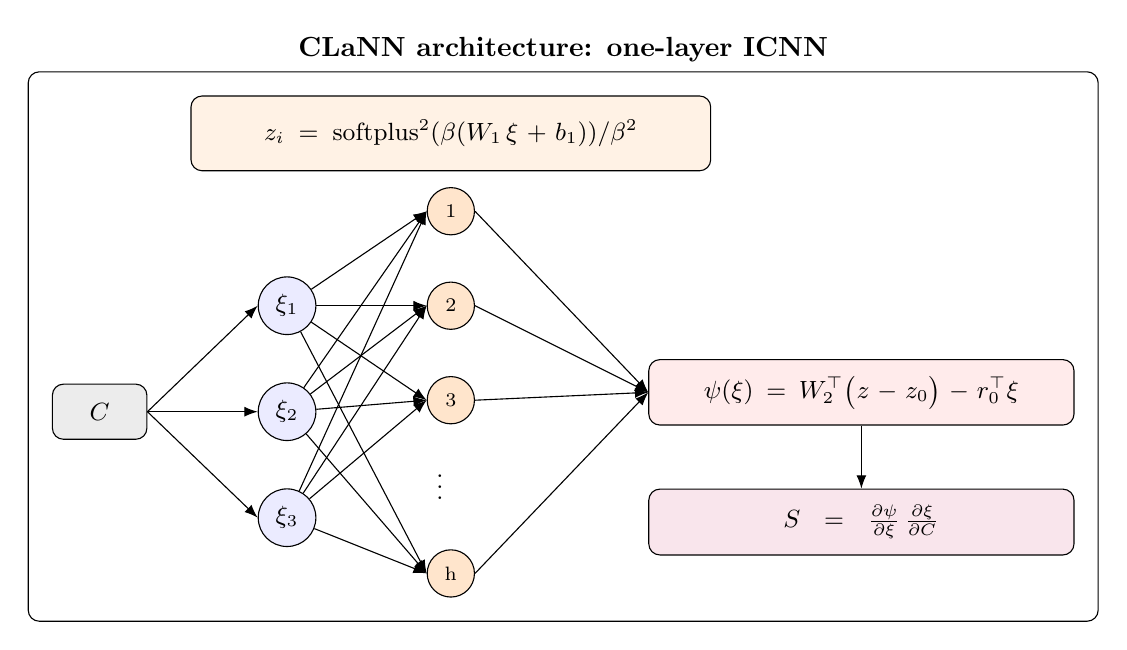
\begin{tikzpicture}[
  font=\small, node distance=9mm and 14mm, >={Latex},
  box/.style={draw, rounded corners, align=center, minimum height=7mm, inner sep=2mm},
  % цветовые стили
  block/.style={box, fill=green!6, text width=44mm},
  pin/.style={circle, draw, minimum size=6mm, fill=blue!8},
  neur0/.style={circle, draw, minimum size=6mm, fill=orange!20},
  neur/.style={circle, draw, minimum size=6mm, fill=orange!20},
  cblk/.style={box, fill=gray!15, text width=8mm},
  actblk/.style={box, fill=orange!10, text width=60mm, inner sep=3mm},
  readblk/.style={box, fill=red!8, text width=50mm},
  gradblk/.style={box, fill=purple!10, text width=50mm},
  title/.style={font=\bfseries},
  every fit/.style={draw, rounded corners, inner sep=3mm}
]


% Входы (лог‑лапласовы координаты)
\node[pin] (x1) {$\xi_1$};
\node[pin, below=6mm of x1] (x2) {$\xi_2$};
\node[pin, below=6mm of x2] (x3) {$\xi_3$};
% Блок правее Cauchy–Green тензора C
\node[cblk, left=14mm of x2] (C) {$\mathbb{C}$};
\draw[->] (C.east) -- (x1.west);
\draw[->] (C.east) -- (x2.west);
\draw[->] (C.east) -- (x3.west);

% Аффинная проекция
\node[neur0, right=14mm of x1, yshift=12mm] (h11) {\scriptsize 1};
\node[neur0, right=14mm of x1] (h12) {\scriptsize 2};
\node[neur0, right=14mm of x1, yshift=-12mm] (h13) {\scriptsize 3};
\node[align=center, right=14mm of x1, yshift=-22mm] (vdots0) {$\vdots$};
\node[neur0, right=14mm of x1, yshift=-34mm] (h14) {\scriptsize h};
\draw[->] (x1) -- (h11.west);
\draw[->] (x2) -- (h11.west);
\draw[->] (x3) -- (h11.west);
\draw[->] (x1) -- (h12.west);
\draw[->] (x2) -- (h12.west);
\draw[->] (x3) -- (h12.west);
\draw[->] (x1) -- (h13.west);
\draw[->] (x2) -- (h13.west);
\draw[->] (x3) -- (h13.west);
\draw[->] (x1) -- (h14.west);
\draw[->] (x2) -- (h14.west);
\draw[->] (x3) -- (h14.west);
% \node[block, above=2mm of h11, text width=36mm] (aff) {$s = W_1\,\xi + b_1$};
\node[actblk, above=2mm of h11] (soft) {$z_i = \mathrm{softplus^2}(\beta (W_1\,\xi + b_1))/\beta^2$};

% % Скрытый слой (softplus): три нейрона, троеточие и ещё один
% \node[neur, right=14mm of h12, yshift=12mm] (h1) {};
% \node[neur, right=14mm of h12] (h2) {};
% \node[neur, right=14mm of h12, yshift=-12mm] (h3) {};
% \node[align=center, right=14mm of h12, yshift=-22mm] (vdots1) {$\vdots$};
% \node[neur, right=14mm of h12, yshift=-34mm] (h4) {};
% \draw[->] (h11.east) -- (h1.west);
% \draw[->] (h12.east) -- (h2.west);
% \draw[->] (h13.east) -- (h3.west);
% \draw[->] (h14.east) -- (h4.west);
% % Блок активации над нейронами
% \node[block, above=2mm of h1, text width=36mm] (soft) {$z_i = \mathrm{softplus}(\beta (W_1\,\xi + b_1)/\beta$};

% Линейный выход (неотрицательные веса), центрирован относительно столбца нейронов
\node[readblk, right=22mm of h12, yshift=-11mm] (readout) {$\psi(\vect{\xi}) = \vect{W}_2^{\top}\big(z - z_0\big) - \vect{r}_0^{\top}\vect{\xi}$};
\draw[->] (h11.east) -- (readout.west);
\draw[->] (h12.east) -- (readout.west);
\draw[->] (h13.east) -- (readout.west);
\draw[->] (h14.east) -- (readout.west);

% Производная: второй тензор Пиолы–Кирхгофа
\node[gradblk, below=8mm of readout] (Sblock) {$\mathbb{S} = \frac{\partial \psi}{\partial \vect{\xi}}\, \frac{\partial \vect{\xi}}{\partial \mathbb{C}}$};
\draw[->] (readout.south) -- (Sblock.north);

% % Центрирование \to физическая энергия
% \node[block, below=10mm of readout] (psiphys) {$\psi_{\mathrm{phys}}(\boldsymbol{\xi}) = \psi(\boldsymbol{\xi}) - \mathbf{r}_0^{\top}\boldsymbol{\xi}$ \\
%   \scriptsize $r_0 = W_1^{\top}\!(w_2^{+}\!\odot\!\sigma(\beta b_1))$};
% \draw[->] (readout.south) -- (psiphys.north);

% Рамка и заголовок
\node[fit=(C)(h14)(soft)(readout)(Sblock), label={[title]above:{CLaNN architecture: one-layer ICNN}}] (archfit) {};

\end{tikzpicture}}
  \caption{Schematic of the CLaNN architecture.}
  \label{fig:clann_arc}
  \label{fig:clann_icnn1_nn}
\end{figure}

\begin{figure}[H]
  \centering
  \resizebox{\textwidth}{!}{% ======= CLaNN: FE stretch -> dataset -> CLaNN arch (vertical) -> S -> Train -> (g,H) -> FE inflation =======
% Требует: \usepackage{tikz} \usetikzlibrary{arrows.meta,positioning,fit}
\begin{tikzpicture}[
  font=\small, node distance=8mm and 14mm, >={Latex},
  box/.style={draw, rounded corners, align=center, minimum height=8mm, inner sep=2mm},
  thinbox/.style={draw, rounded corners, align=center, minimum height=6mm, inner sep=1.2mm, text width=52mm},
  inpin/.style={circle, draw, minimum size=5.2mm},
  hid/.style={circle, draw, minimum size=6mm},
  title/.style={font=\bfseries},
  dashedarrow/.style={->, dashed},
  boxL/.style={box, fill=blue!6},
  boxM/.style={box, fill=green!6},
  boxR/.style={box, fill=orange!10},
  trainbox/.style={box, fill=purple!8}
]

% ---------------- Simplified pipeline (3 columns, orthogonal arrows) ----------------
% LEFT COLUMN
\node[boxL, minimum width=46mm, minimum height=32mm] (fe) {FE stretching\\ \scriptsize protocols $p$\\[2pt]
  \includegraphics[width=0.3\linewidth]{../img/Numerical/malt_stress.png}};
\node[boxL, below=8mm of fe, minimum width=46mm] (data) {Data collection\\ $D(p,w)=\{(\mathbb{C},\mathbb{S})\}$};

% MIDDLE COLUMN
\node[boxM, right=28mm of fe, minimum width=54mm] (xi) {Laplace strain\\ $\boldsymbol{\xi}=\boldsymbol{\xi}(\mathbb{C})$};
\node[boxM, below=8mm of xi, minimum width=54mm] (arch) {CLaNN architecture\\ $\psi_{\rm phys}(\boldsymbol{\xi})$};
\node[boxM, below=8mm of arch, minimum width=54mm] (smap) {Autodiff \\[1pt] $\displaystyle \hat{\mathbb S}=\frac{\partial\psi_{\rm phys}}{\partial \mathbb{C}}$};
\node[trainbox, below=8mm of smap, minimum width=54mm] (train) {Training\\ $L=\|\hat{\mathbb S}-\mathbb S\|_{L2}\xrightarrow{\text{Adam}}0$};

% RIGHT COLUMN
\node[boxR, right=28mm of arch, minimum width=50mm] (gh) {Derivatives\\ $g(\boldsymbol{\xi}),\ H(\boldsymbol{\xi})$};
\node[boxR, below=8mm of gh, minimum width=50mm, minimum height=36mm] (infl) {FE inflation tests \\ homogeneous / heterogeneous thickness \\[2pt]
  \includegraphics[width=0.3\linewidth]{../img/Numerical/het/plane.png}};

% ORTHOGONAL ARROWS
\draw[->] (fe) -- (data);
% вилка от датасета: одна ветвь к деформации, другая — к обучению
\path (data.east) -- ++(10mm,0) coordinate (datasplit);
\draw[->] (data.east) -- (datasplit) |- (xi.west);
\draw[->] (datasplit) |- (train.west);
\draw[->] (xi) -- (arch);
\draw[->] (arch) -- (smap);
\draw[->] (smap) -- (train);
\draw[->] (arch.east) -- (gh.west);
\draw[->] (gh.south) -- (infl.north);
% пунктир: обновление параметров из обучения обратно в архитектуру (слева)
\draw[dashedarrow] (train.west) -- ++(-8mm,0) |- (arch.west);

\end{tikzpicture}
}
  \caption{Schematic of the CLaNN computational loop.}
  \label{fig:clann_pipeline}
\end{figure}

This CLaNN architecture ensures all necessary physical properties of the hyperelastic model: 
\textbf{thermodynamic consistency} is achieved through strict compliance with \eqref{eq:chain-rule}, 
which guarantees conservative stresses $\oint \mathbb{S}:\mathrm{d}\mathbb{C} = 0$ and consistency with the laws of 
thermodynamics; 
\textbf{Stress objectivity} holds automatically thanks to the parametrization via the 
Cauchy--Green tensor $\mathbb{C} = \mathbb{F}^{\top}\mathbb{F}$, ensuring invariance with respect to rotations and stress symmetry; 
\textbf{strict non-negativity and coercivity of the energy} are provided by the architectural calibration 
$\psi_{\mathrm{phys}}(\boldsymbol{\xi}) = \mathbf{W}_2^{\top}(z - z_0) - \mathbf{r}_0^{\top}\boldsymbol{\xi}$,
yielding $\psi_{\mathrm{phys}}(\mathbf{0})=0$, $\psi_{\mathrm{phys}}(\boldsymbol{\xi})>0$ for $\boldsymbol{\xi}\ne\mathbf{0}$ and 
$\psi_{\mathrm{phys}}(\boldsymbol{\xi})\to\infty$ as $\|\boldsymbol{\xi}\|\to\infty$; 
finally, the \textbf{physical constraints} \eqref{eq:energy_constraints} are satisfied by the CLaNN network design: monotone, convex activations,
nonnegative output weights, and centering of the strain energy $\psi$ and the response $\vect r$.




% Virtual experiment / Results
% \section{Virtual Experiment}
\section{Виртуальный эксперимент}

Для обучения и тестирования CLaNN мы использовали синтетические  данные двухосного растяжения и раздувания гиперупругой мембраны соответственно.
% Мы используем синтетические экспериментальные данные для тестирования CLaNN 
% на изотропном надуваним однородной и неоднородной по толщине мембраны. 
% А именно, мы генерируем данные с помощью виртуальных экспериментов на плоских растяжениях образца и используем их в качестве входных данных для 
% обучения CLaNN, без какого-либо дополнительного знания об изотропности/анизотропности образца и форме потенциала.
Обучение модели проводилось на численных экспериментальных данных, 
полученных при двухосном растяжении образца с геометрией "мальтийский крест" и толщиной $H=0.53$ мм (Рисунок \ref{fig:malt_geometry}) методом гиперупругой узловой силы \cite{ddaniso2024}. 
Материал мембраны задавался неогуковской моделью \cite{ogden1997nonlinear}:
\begin{align} \label{eq:neohook}
        \widetilde{\psi} &= \dfrac{\mu H(X)}{2} (I_1 +J^{-2}-3),
        \quad     I_1 = e^{2\xi_1} (1+\xi_3^2)+e^{2\xi_2},\quad J = e^{\xi_1+\xi_2}
\end{align}
с $\mu=0.43\cdot 10^6$ Па.

% Данные для обучения извлекались из различных областей образца...

% Для решения задачи равновесия гиперупругой мембраны используется метод описанный в \cite{ddaniso2024}.

\begin{figure}[H]
  \centering
  \includegraphics[width=0.4\textwidth]{img/malt_geom.png}
  \caption{Геометрия образца}
  \label{fig:malt_geometry}
  \label{fig:malt_displacements}
\end{figure}

Схема нагружения образца показана на рисунке \ref{fig:malt_displacements}, где $w_i \in [0,1]$, $i \in \{1,4\}$
представляет собой долю от заданного максимального смещения $u_{\max}$ для $i$-го плеча: $w_i = 0$ 
соответствует неподвижному плечу, а $w_i = 1$ — соответствует плечу, чьё положение было сдвинуто и фиксировано на расстояние $u_{max}$. 
Изменяя $w_i$, можно получить различные варианты двухосного нагружения. 
В наших виртуальных экспериментах мы последовательно
смещаем плечи с приращением $\Delta s$. 
Смещение $w_i \cdot n \cdot \Delta s$ прикладывается к $i$-му плечу на $n$-м шаге, где $n = 1, \ldots, N$, 
$N = u_{\max}/\Delta s$ — количество шагов. 
Метод гиперупругой узловой силы применялся к изначально плоской квазиоднородной неструктурированной триангуляции с шагом сетки $h=0.5$ мм и размером $5 404$ треугольников. Максимальное смещение плеча
$u_{\max} = 2$ мм и $\Delta s = 0.2$ мм.
На каждом шаге извлекались $\mathbb{C}, \mathbb{S}$ для всех треугольников, принадлежащих выбранной области наблюдения. 
% Поскольку мы используем линейные ($P_1$) конечные элементы, значения $(\\mathbb C, \\mathbb S)$ постоянны на каждом треугольнике.

 
 
Наш предлагаемый тестовый протокол предполагает девять экспериментов:

\begin{figure}[H]
  \centering
  \begin{minipage}[t]{0.48\textwidth}
    \centering
    \vspace{0pt}
    \begin{tabular}{|c|c|c|c|c|}
    \hline
    \textbf{№} & $w_1$ & $w_2$ & $w_3$ & $w_4$ \\
    \hline
    1 & 1 & 1 & 1 & 1 \\
    2 & 1 & 0.75 & 1 & 0.75 \\
    3 & 0.75 & 1 & 0.75 & 1 \\
    4 & 1 & 0.5 & 1 & 0.5 \\
    5 & 0.5 & 1 & 0.5 & 1 \\
    6 & 1 & 1/3 & 1 & 1/3 \\
    7 & 1/3 & 1 & 1/3 & 1 \\
    8 & 1 & 0 & 1& 0 \\
    9 & 0 & 1 & 0 & 1 \\
    \hline
    \end{tabular}
    \captionof{table}{Протоколы тестовых экспериментов}
    \label{tab:test_protocols}
  \end{minipage}\hfill
  \begin{minipage}[t]{0.48\textwidth}
    \centering
    \vspace{0pt}
    \includegraphics[width=\linewidth]{img/Numerical/malt_window.pdf}
    \captionof{figure}{Поле напряжения $\vect S$ деформированной мембраны с геометрией "мальтийский крест" с различными окнами наблюдения $w$.}
    \label{fig:malt_window}
  \end{minipage}
\end{figure}

\subsubsection{Правила отбора данных}
\paragraph{Центральное окно $w$.}
Окно задаётся в исходной конфигурации $\Omega_0$ как центральная область вокруг геометрического центра 
образца, согласованная с осями расчётной сетки.
Для $w=5\times5$ мм и $w=10\times10$ мм берётся квадрат со сторонами 5 и 10 мм соответственно, 
центрированный в центре образца; для $w=\text{всё поле}$ — вся область $\Omega_0$.
Для $w=\text{1-элемент}$ берётся единственный центральный треугольник 
(ячейка с минимальным номером на вычислительной сетке для окна 5x5 мм $\Omega_0$ как показано на рисунке \ref{fig:malt_window} ).
Наблюдения включают все треугольники, барицентры которых $\mathbf{X}_T$ лежат внутри выбранного окна $\mathcal{W}_w\subset\Omega_0$.
% TODO: добавить мощность окна в элементах сетки

\paragraph{Состав наблюдений (данные).}
На каждом шаге нагружения $n=1,\dots,N$ и для каждого треугольника $T\in\mathcal{T}_w$ (ячейки, попавшие в окно) фиксируется пара $(\mathbb C_T^{(n)},\,\mathbb S_T^{(n)})$, 
где $\mathbb C$ — правый тензор Коши–Грина, $\mathbb S$ — второй тензор Пиолы–Кирхгофа.
Единицы: размеры окна — мм; $\mathbb C$ — безразмерен; $\mathbb S$ — МПа. 
При этом количество элементов сетки в окне наблюдения $|\mathcal{T}_w|$ для различных окон различно: 
$1$ для $w=\text{1-элемент}$, $252$ для $w=5\times5$ мм, $954$ для $w=10\times10$ мм и $5404$ для $w=\text{всё поле}$.

\paragraph{Формирование выборок.}
Для фиксированных $(p,w)$ совокупность всех пар $(\mathbb C_T^{(n)},\,\mathbb S_T^{(n)})$ образует базовый набор $D(p,w)$, из которого формируются разбиения $D_{\mathrm{tr}}(p,w)$ и $D_{\mathrm{val}}(p,w)$.
Для заданных протокола $p$ (см. табл.~\ref{tab:test_protocols}) 
и окна центральной области образца 
$w\in\{\text{1-элемент},\,5\times5\,\text{мм},\,10\times10\,\text{мм},\,\text{всё поле}\}$ обозначим
\[
  D_{\mathrm{tr}}\equiv D_{\mathrm{tr}}(p,w),\qquad D_{\mathrm{val}}\equiv D_{\mathrm{val}}(p,w),
\]
где $D_{\mathrm{tr}}$ — обучающая, $D_{\mathrm{val}}$ — валидационная выборки.



Например, |D(\{1..10\}, \text{1-элемент})|= 90 точек данных правого тензора деформаций Коши-Грина $\mathbb C$ 
и второго тензора напряжений Пиолы-Кирхгофа $\mathbb S$ (Рисунок \ref{fig:training_data}).

\begin{figure}[H]
  \centering
  \includegraphics[width=1.0\textwidth]{img/all_stress_plots.png}
  \caption{Обучающий набор данных}
  \label{fig:training_data}
\end{figure}

Так как мы собираем данные из одного центрального элемента сетки, то растягивающие компоненты $xx, yy$ тензоров деформации $\mathbb C$ и напряжения
$\mathbb S$ имеют значения на 2-3 порядка большие чем сдвиговые компоненты $xy$.

\subsubsection{Метрики и критерии качества}
\label{sec:metrics}

Для количественной оценки качества предсказаний используем интегральные и точечные метрики, согласующиеся с энергетической нормой из вариационной постановки задач упругости (см., например, \cite{ciarlet1988mathematical,ogden1997nonlinear,holzapfel2000nonlinear}).

\textbf{Коэффициент детерминации $R^2$.}
\begin{equation}\label{eq:r_squared}
  R^2 = 1 - \frac{\sum_{i=1}^n (y_i - \hat{y}_i)^2}{\sum_{i=1}^n (y_i - \bar{y})^2},
\end{equation}
где $y_i$ — экспериментальные значения, $\hat{y}_i$ — предсказания модели, $\bar{y}$ — среднее экспериментальных значений, $n$ — число точек. Назначение: удобно сравнивать кривые нагружения; даёт нормированную меру согласия по траекториям.

\textbf{Точечная относительная ошибка.}
\begin{equation}\label{eq:rel_error}
  \epsilon = \frac{\| \mathbb S - \mathbb S_{\text{ref}} \|}{\| \mathbb S_{\text{ref}} \|}.
\end{equation}
% Назначение: отрисовка поля ошибки и его локальной структуры; наглядна на картах.

\textbf{P1-ошибка} \cite{xie2024p1} — комбинация абсолютной и относительной ошибок, чувствительная к малым значениям:
\begin{equation}\label{eq:p1_error}
  \epsilon_{\mathrm{P1}} = \frac{\| \mathbb S - \mathbb S_{\text{ref}} \|}{s_0 + \| \mathbb S_{\text{ref}} \|},\qquad s_0 = \max(\mathbb S_{\text{pred}}).
\end{equation}

\textbf{Абсолютная интегральная ошибка (L2 по сетке) для напряжений (Фробениус-норма).}
\begin{equation}\label{eq:l2_abs_stress}
  \|e\|_{L^2} = \Bigg( \sum_{K} \overline{\| \mathbb S_{\text{ref}} - \mathbb S_{\text{pred}} \|_F^{2}}^{\,K}\, |K| \Bigg)^{\tfrac12},
\end{equation}
где $|K|$ — мера ячейки (объём/площадь/длина). Для ячеечных данных усреднение по ячейке не требуется:
\begin{equation}\label{eq:l2_abs_stress_cell}
  \|e\|_{L^2} = \Bigg( \sum_{K} \| \mathbb S_{\text{ref},K} - \mathbb S_{\text{pred},K} \|_F^{2}\, |K| \Bigg)^{\tfrac12}.
\end{equation}
Назначение: сворачивает поле ошибки в скаляр и инвариантна к измельчению сетки (при фиксированном поле) \cite{BrennerScott2008,AinsworthOden2000,Verfurth2013}.

\textbf{Относительная интегральная ошибка.}
\begin{equation}\label{eq:l2_rel_stress}
  \|e\|_{L^2,\,\mathrm{rel}}\;=\; \frac{\Big( \sum\limits_{K} 
  \| \mathbb S_{\mathrm{ref},K} - \mathbb S_{\mathrm{pred},K} \|_F^{2}\, |K| \Big)^{\tfrac12}}
  {\Big( \sum\limits_{K} \| \mathbb S_{\mathrm{ref},K} \|_F^{2}\, |K| \Big)^{\tfrac12}}\,.
\end{equation}
% Назначение: корректное сопоставление сценариев с разными уровнями напряжений; нормировка на «энергетическую мощность» эталонного поля.


\textbf{Гиперпараметры оптимизации:}
\begin{itemize}
  \item Скорость обучения (learning rate): $0.001$
  \item Размер батча (batch size): $4$ при обучении на 90 точек данных и $128$ для остальных обучающих наборов данных.
  % \item Веса физических ограничений: $\lambda_{\text{SI}} = 0.1$, $\lambda_{\psi} = 0.1$
  \item Архитектура: 16 нейронов на скрытом слое
  \item Сглаживающий параметр $\beta$: $10$
\end{itemize}

\textbf{Результаты обучения:}
Процесс оптимизации показал высокую эффективность: ошибка аппроксимации снизилась на 5 порядков за менее чем 5000 эпох (рисунок \ref{fig:loss_curve}), 
что демонстрирует как качество предложенной архитектуры, так и корректность выбора гиперпараметров. 
Столь быстрая сходимость обусловлена строгой выпуклостью функции энергии, что обеспечивает единственность 
минимума и отсутствие локальных минимумов в пространстве параметров.

\begin{figure}[H]
  \centering
  \includegraphics[width=0.7\textwidth]{img/loss_curve.png}
  \caption{Кривая функции потерь при обучении на 90 точках данных}
  \label{fig:loss_curve}
\end{figure}


\subsection{Интерполяция и экстраполяция кривых нагружения}
  Сначала мы проверили, как модель CLaNN интерполирует и экстраполирует кривые нагружения, используя выборки
  $D_{\mathrm{tr}}(p,w)$ и $D_{\mathrm{val}}(p,w)$ для заданного окна наблюдения $w$.
  Для оценки качества использовали коэффициент детерминации $R^2$ (см. раздел \ref{sec:metrics}, формулу \eqref{eq:r_squared}). Метрику качества фиксируем как:
\[
  R^2_{\alpha}(D_{\mathrm{val}}),\qquad \alpha\in\{xx,yy,xy\}.
\]

  \textbf{Интерполяция.}  

  Для тестирования способности архитектуры CLaNN к интерполяции кривых нагружения мы использовали данные из 
  10 точек кривой нагружения равнодвухосного растяжения мембраны $p=1$, 
  окно наблюдения $w=\text{1-элемент}$:
  
  $D_{in} = D(p{=}1,\,w{=}\text{1-элемент}),\, n = 1..10,$
  
  $D_{\mathrm{tr}}=\{\forall (\mathbb {C}^{n_{tr}}, \mathbb{S}^{n_{tr}}) \in D_{in}|\; n_{tr}=\{1,5,10\}\},$
  
  $D_{\mathrm{val}}=\{\forall (\mathbb {C}^{n_{val}}, \mathbb{S}^{n_{val}}) \in D_{in}|\; n_{val}=n \\  n_{tr}\}.$

  CLaNN показал высокую точность интерполяции кривой нагружения равнодвухосного растяжения мембраны 
  для растягивающих компонент $R^2_{xx}=0.999$, $R^2_{yy}=0.999$, и отсуствие достоверного предсказания сдвиговых 
  компонент $R^2_{xy}=0$ (рисунок \ref{fig:interpolation}).
  
  \begin{figure}[H]
    \centering
    \includegraphics[width=1.0\textwidth]{img/interpolation.png}
    \caption{Кривая нагружения для равнодвухосного растяжения}
    \label{fig:interpolation}
  \end{figure}
  
  \textbf{Экстраполяция.}
  
  Для проверки способности CLaNN к экстраполяции кривых нагружения использовали обучение на равнодвухосном растяжении (p = 1) и валидацию на неравнодвухосном (p = 9), 
  окно наблюдения $w=\text{1-элемент}$:
  
  $D_{\mathrm{tr}} = D(p{=}1,\,w{=}\text{1-элемент}),\, n = 1..10,$
  
  $D_{\mathrm{val}} = D(p{=}9,\,w{=}\text{1-элемент}),\, n = 1..10,$
  
  CLaNN показал высокую точность экстраполяции для растягивающих компонент $R^2_{xx}=0.993$, $R^2_{yy}=1.0$, и отсутствие достоверного предсказания сдвиговой компоненты $R^2_{xy}=0$ (рисунок \ref{fig:extrapolation}).


  \begin{figure}[H]
    \centering
    \includegraphics[width=1.0\textwidth]{img/extrapolation.png}
    \caption{Кривая нагружения для неравнодвухосного растяжения}
    \label{fig:extrapolation}
  \end{figure}
   
  Таким образом, CLaNN способен интерполировать и экстраполировать кривые нагружения с высокой точностью, что свидетельствует о его способности к обобщению на новые данные.
  Однако, не справляется с предсказанием сдвиговых компонент $\mathbb S_{xy}$, что может быть связано с тем, что данные для сдвиговых компонент не достаточно большие.
  
  Проблему недостатка данных для обучения модели CLaNN на сдвиговых компонентах деформации/напряжения мы обсудим дальше.
\subsection{Раздутие мембраны}

  Для проверки описательной и предсказательной способностей CLaNN, мы поставили численный эксперимент по раздутию круглой мембраны радиусом 25 мм.
  Мембрана закреплена по внешнему контуру и подвергается равномерному растяжению по всей поверхности при заданном давлении
  5 МПа. 
  Как референс мы использовали результаты численного эксперимента с использованием гиперупругой модели Нео-Гука с тем же параметром сдвига, 
  что и при генерации данных для обучения CLaNN.
  
  Мы использовали два поля толщин элементов $T$: 1) с гомогенным полем толищны 0.54 мм. 
  2) с гетерогенным полем толищны, где в в окружности высекается два пораболических сектора с толщиной 2 мм
  и остальной части мембраны 0.54 мм (Рисунок \ref{fig:membrane_thickness}). 

  В качестве точечной метрики используем относительную ошибку (см. раздел \ref{sec:metrics}, формулу \eqref{eq:rel_error});
  для сравнения сдвиговых компонент — P1-ошибку \cite{xie2024p1} (см. формулу \eqref{eq:p1_error}).

  \begin{figure}[H]
    \centering
    \includegraphics[width=0.25\linewidth]{img/het_circle.png}
    \caption{Гетерогенное поле толщин элементов $T$ круглой мембраны.}
    \label{fig:membrane_thickness}
  \end{figure}
  % \begin{wrapfigure}{r}{0.35\textwidth}
  %   \centering
  %   \includegraphics[width=\linewidth]{img/het_circle.png}
  %   \caption{Гетерогенное поле толщин элементов $T$ круглой мембраны.}
  %   \label{fig:membrane_thickness}
  % \end{wrapfigure}
  % Для геометрии с гетерогенным полем толщин референсные значения сдвиговой компоненты поля 2 тензора напряжений Пиолы-Кирхгофа 
  % $\vect S$ (Рисунок \ref{fig:numerical_experiment}) .

  \begin{figure}[H]
    \centering
    \includegraphics[width=0.7\textwidth]{img/Numerical/ref_stress.png}
    \caption{Поле напряжений $\mathbb S$ круглой мембраны (пример результата численного эксперимента).}
    \label{fig:numerical_experiment}
  \end{figure}
  
  В результате численного эксперимента на раздутие мембраны с гиперупругим определяющим соотношением CLaNN,
  используя набор данных $D (\{1..10\}, w=\text{1-элемент})$ для обучения, мы получили поле напряжений 2 тензора Пиолы-Кирхгофа 
  $\mathbb S$ для гомогенной и гетерогенной мембраны по толщине и сравнили его
  с референсными значениями (Рисунок \ref{fig:numerical_experiment}) и построили поле ошибок $\epsilon$ и $\epsilon_{P1}$ (Рисунок \ref{fig:numerical_errors}).
  Сдвиговая компонента напряжений $\mathbb S_{xy}$ показывает наибольшую ошибку для гетерогенной мембраны, 
  что может быть связано с тем, что данные для сдвиговых компонент не достаточно большие. Поэтому мы последовательно 
  расширяли набор данных для обучения до $D (\{1..10\}, w=\text{5x5})$, $D (\{1..10\}, w=\text{10x10})$, $D (\{1..10\}, w=\text{все поле})$, 
  и построили зависимость интегральной ошибки $\|e\|_{L^2}$ (Формула \ref{eq:l2_abs_stress_cell}) и $\|e\|_{L^2,\,\mathrm{rel}}$ (Формула \ref{eq:l2_rel_stress}) 
  поля напряжения $\mathbb S$ от размера окна наблюдения $w$ (Рисунок \ref{fig:integral_errors}). 
  В итоге абсолютная интегральная ошибка $\|e\|_{L^2}$  для гетерогенной мембраны уменьшается с увеличением размера окна наблюдения $w$, 
  это может быть связано с тем, что при увеличении размера окна наблюдения мы учитываем больше данных для обучения, в том числе данных 
  для сдвиговых компонент напряжений, например, при отборе ячеек из области ближе к углам квадрата, в который вписана мембрана, 
  сдвиговые компоненты напряжений в этой области вырастают на 1-2 порядка.
  
  
  \begin{figure}[H]
    \centering
    \includegraphics[width=1.0\textwidth]{img/Numerical/errs.png}
    \caption{Поле ошибок между предсказанными и эталонными значениями напряжений.}
    \label{fig:numerical_errors}
  \end{figure}

  \begin{figure}[H]
    \centering
    \includegraphics[width=0.5\textwidth]{img/integral_errors.png}
    \caption{Зависимость интегральной ошибки $\|e\|_{L^2}$ и $\|e\|_{L^2,\,\mathrm{rel}}$ от количества элеметов в окне наблюдения размера $w$.}
    \label{fig:integral_errors}
  \end{figure}
  
  % \begin{figure}[H]
  %   \centering
  %   \includegraphics[width=0.7\textwidth]{img/integral_errors.png}
  %   \caption{Интегральные ошибки в зависимости от окна наблюдения.}
  %   \label{fig:_integral_numerical_errors}
  % \end{figure}
  
\subsection{Сравнение вычислительной эффективности CLaNN}

  Благодаря \emph{выпуклости} потенциальной энергии деформации $\psi(\boldsymbol\xi)$ в CLaNN задача стационарного равновесия формулируется
  как гладкая выпуклая минимизация. Это позволяет использовать градиентные и второпорядковые методы со строгими гарантиями сходимости
  (квазиньютон, Ньютона и тд)
  и предсказуемой сложностью до заданной точности \cite{BoydVandenberghe2004,Nesterov2004,NocedalWright2006,ConnGouldToint2000}.
  В окрестности минимума сильная выпуклость и липшицевость гессиана обеспечивают локально квадратичную сходимость Ньютона,
  а квазиньютоновские схемы (L\textendash BFGS) дают сверхлинейные скорости \cite{NocedalWright2006}.

  % \paragraph{Data-drevin модели без выпуклости.}
  В таблично-заданных/локально-интерполяционных DD-моделях (в т.ч.\ k-NN, IDW) выпуклость энергии, как правило, не гарантируется,
  а функция отклика может быть негладкой. Это приводит к невыпуклой постановке с множеством стационарных точек и
  отсутствием глобальных гарантий у классических квазиньютоновских методов. На практике применяются
  квазистатические/релаксационные стратегии: (добавить описание) \cite{KirchdoerferOrtiz2016,KirchdoerferOrtiz2017}.
  Такие методы устойчивы, но, как правило, требуют существенно большего числа шагов нагружения и внутренних итераций
  (а также повторяющихся k-NN/IDW-запросов), что приводит к росту времени расчёта.

  Мы сравнили время решения для CLaNN, классической гиперупругой модели Нео\textendash Гука и DD-модели мембраны, описанной в \cite{xi2023}.
  Задача: раздувание закреплённой круглой мембраны, $R{=}25$ мм, равномерное давление, две конфигурации по толщине $T$ (гомогенная и гетерогенная; см. рис.~\ref{fig:membrane_thickness}).
  Для CLaNN обучаем на наборе данных $D(\{1..10\},\,w{=}\text{1-элемент})$; для сравнения используем DD-модель на основе 
  kNN и IDW, которые работает в пространстве деформаций Лапласа и функций отклика $(\vect{\xi}, \vect{r})$, 
  которые были вычислены из $D(\{1..10\},\,w{=}\text{10}\times\text{10})$ \cite{xi2023}.
  Численное решение выполняем в одной и той же КЭ-постановке для мембранной задачи. 
  Все варианты останавливаем по одинаковым нормам допускам по невязке.

\begin{table}[htbp]
\centering
\caption{Время расчёта (сек) на задаче раздувания: гомогенная vs гетерогенная толщина}
\label{tab:experiments_summary}
\begin{tabular}{|l|c|c|}
\hline
\textbf{Метод} & \textbf{Гомогенная} & \textbf{Гетерогенная} \\
\hline
CLaNN & 512 & 329  \\
\hline
Neo-Hooke & 13 & 16\\
\hline
kNN & 993 & -- \\
\hline
\end{tabular}
\end{table}

  На одинаковой сетке и допусках CLaNN достигает решения сравнимым числом глобальных итераций с Нео\textendash Гуком
  (за счёт выпуклости и корректной кривизны энергии в ICNN), но большим итоговым вычислительным временем, что связано с низкой вычислительной эффективностью 
  взаимодействия экспортируемой модели CLaNN и мембранного решателя \cite{xi2023}.
  Метод CLaNN существенно опережает DD-модель по времени расчета
  за счёт отсутствия внешних проекций на данные и дорогих k-NN/IDW-запросов на каждой итерации.
  Также стоит отметить невозможность расчета DD-модели на гетерогенной толщине без линейной интерполяции данных в близи нуля, 
  что может происходить из-за нехватки данных для этой области деформаций.




% Conclusions
% \section{Conclusion}


\section{Дискуссия}

В данной работе предложена и реализована физически-информированная архитектура CLaNN для гиперупругих материалов, основанная на выпуклой потенциальной энергии деформации и меры деформации Лапласа.

В исследованиях по основанной на данных механике \cite{KirchdoerferOrtiz2016,salamatova2020hyperelastic} отклик строится как локальная интерполяция (Voronoi, k-NN) в пространствах деформаций-напряжений, что ведет к невыпуклой задаче равновесия и необходимости применения релаксационных стратегий решения, вместо градиентных и второпорядковых методов со строгими гарантиями сходимости (квазиньютоновские схемы, Ньютон и т.д.). Такие методы устойчивы, но, как правило, требуют существенно большего числа шагов нагружения и внутренних итераций (а также повторяющихся k-NN/IDW-запросов), что приводит к росту времени расчёта. 

Локальную интерполяцию мы заменили интерполяцией таблично-заданного в мерах Лапласа определяющего соотношения \cite{salamatova2020hyperelastic} выпуклым по входу нейропотенциалом на базе ICNN. Такой подход априори удовлетворяет требованию к объективности, материальной симметрии \cite{freed2020laplace}, симметрии тензора напряжения и выпуклости гиперупругой модели. Последнее достигалось архитектурно, через монотонно неубывающую функцию активации и неотрицательные веса в соответствии с \cite{icnn2017}. Для построения гиперупругой модели CLaNN мы провели виртуальный аналог двухосного экспериментального исследования (по протоколу из \cite{sommer2015biomechanical}) крестообразного образца неогуковского материала. Входными данными для обучения модели CLaNN стали пары деформация-напряжение $\boldsymbol{\xi}_r^{(n)}, \mathbb{S}_r^{(n)}$, извлеченные из виртуального эксперимента. Полученная модель продемонстрировала высокую точность интерполяции для главных компонент напряжений при растяжении обучающих данных.

В работе \cite{tacc2024benchmarking} авторы сравнивают подходы к моделированию гиперупругости физически-информированными архитектурами CANN (Constitutive Artificial Neural Networks), ICNN (Input Convex Neural Networks), NODE (Neural Ordinary Differential Equations). Для изотропных эластомеров (при одноосных, равнодвухосных, сдвиговых модах дефомирования) показано, что обучение физически дополненных сетей на равнодвухосном растяжении обеспечивает лучшую межрежимную экстраполяцию. Подобным образом мы протестировали экстраполяционную способность трех вариантов CLaNN, обученных на данных сложного двухосного протокола, извлеченных из разных областей образца. Моделировалось два инфляционных сценария -- раздувание гомогенной по толщине мембраны и гетерогенной мембраны с утолщениями-концентраторами, продуцирующими неоднородные поля деформаций со значительными сдвиговыми компонентами тензора напряжений в полюсе образца.
Точность наших решений, полученная с CLaNN, сравнивалась с референтным конечно-элементным решением для раздутия неогуковской модели мембраны с тем же параметром модуля сдвига, с которым генерировались двухосные данные для обучения CLaNN. При сопоставимой с неогуковским решением скоростью CLaNN корректно предсказывает поля перемещений и напряжений при инфляции гомогенной и гетерогенной по толщине круглой гиперупругой мембраны. Абсолютные и относительные интегральные ошибки норм перемещений и напряжений падают при увеличении области извлечения данных для обучения CLaNN -- к дужкам крестообразного образца растет порядок сдвиговой компоненты напряжений. Это соответствует наблюдениям из бенчмарка \cite{tacc2024benchmarking}: с расширением покрытия экспериментальными данными пространства деформаций при обучении CANN/ICNN/NODE, растет точность межрежимной экстраполяции. 

Отметим, что по вычислительной эффективности CLaNN превосходит методы локальной интерполяции: на гомогенной задаче выигрыш составляет
порядка $\times 141.8$ за счёт отсутствия дорогостоящих k\textendash NN/IDW\textendash запросов и внешних проекций на данные на каждой итерации. 
Стоит отметить, что полученная величина выигрыша может быть и выше за счет оптимизации взаимодействия решателя и CLaNN, а также подбора оптимальных гиперпараметров.
На гетерогенной толщине CLaNN сохраняет работоспособность без специальных эвристик, 
тогда как в предыдущей работе \cite{salamatova2020hyperelastic} таблично\textendash заданная гиперупругая модель требует дополнительной регуляризации и/или интерполяции данных в окрестности малых деформаций.
Также из-за отсутствия критерия остановки расчета по норме невязки у релаксационных методов решения задачи равновесия может привести к сложнооценимому увеличению времени расчета по сравнения с ньютоновскими методами, с которыми позволяет работать CLaNN.

В работе \cite{ddaniso2024} была показана применимость таблично-заданных определяющих соотношений в мерах Лапласа для анизотропных биоматериалов. При этом инварианты для описания анизотропии не вводились. Таблично-заданное определяющее соотношение строилось по синтетическим экспериментальным данным, которые были получены с гиперупругой моделью Хользапфеля-Гассера-Огдена \cite{ddaniso2024} для свиной кожи. Трех функций отклика, зависящих от трех соответствующих компонент тензора Лапласа было достаточно для описания механического поведения анизотропного материала в двумерной постановке. Это обнадеживает применение CLaNN для анизотропного материала без введения предположений о симметриях материала, как это недавно делалось родственных работах с ICNN определяющим соотношениям, базирующимся на инвариантах и псевдо-инвариантах правого тензора деформаций Коши-Грина \cite{kalina2025neural}. В будущем мы планируем обучить модель CLaNN на экспериментальных данных, полученных при тестировании перикардиальной ткани.
Как итог, на фоне феноменологических гиперупругих моделей CLaNN не требует предположений о форме потенциала и предлагает гибкость универсального аппроксиматора потенциала при удовлетворении законов термодинамики. На фоне локально интерполяционных подходов, основанных на данных CLaNN возвращает в постановку гладкость и выпуклость энергии, что превращает задачу равновесия в хорошо обусловленную минимизацию с предсказуемой сходимостью и выигрышем по времени.
Ограничения. Наши результаты демонстрируют, что мы можем успешно применять архитектуру CLaNN для моделирования гиперупругой изотропной мембраны. Однако мы столкнулись с некоторыми ограничениями, которые указывают на будущую работу. Во-первых, в данной работе предполагается гиперупругость мембраны. Во-вторых, мы рассматриваем только изотропный случай в двумерных сценариях. В дальнейшем мы расширим применение CLaNN на анизотропию, устранив это ограничение аппроксимацией таблично-заданного определяющего соотношения в мерах Лапласа для анизотропного материала.

In this work we propose and implement a physics‑informed CLaNN architecture for hyperelastic materials, based on a convex strain‑energy potential and the Laplace strain measure.

In data‑driven computational mechanics \cite{KirchdoerferOrtiz2016,salamatova2020hyperelastic}, the material response is often constructed via local interpolation (Voronoi, k‑NN) in strain–stress spaces. This leads to a nonconvex equilibrium problem and necessitates relaxation‑type solution strategies instead of gradient‑based and second‑order methods with strong convergence guarantees (quasi‑Newton schemes, Newton–Raphson, etc.). Such relaxation methods are robust but typically require many more load increments and internal iterations (as well as repeated k‑NN/IDW queries), which increases runtime.

We replace local interpolation of a tabulated constitutive relation in Laplace strain measures \cite{salamatova2020hyperelastic} with an input‑convex neural potential based on ICNN. This approach a priori satisfies objectivity, material symmetry \cite{freed2020laplace}, stress‑tensor symmetry, and convexity of the hyperelastic model. The latter is enforced architecturally via a monotonically nondecreasing activation function and nonnegative weights, in accordance with \cite{icnn2017}. To build the CLaNN hyperelastic model, we performed a virtual analog of a biaxial experimental study (following \cite{sommer2015biomechanical}) on a cruciform specimen of a Neo‑Hookean material. The training inputs for CLaNN were strain–stress pairs, $\boldsymbol{\xi}_r^{(n)}, \mathbb{S}_r^{(n)}$, extracted from the virtual experiment. The resulting model exhibited high interpolation accuracy for the principal stress components under the tensile states included in the training set.

In \cite{tacc2024benchmarking}, the authors compare physics‑informed architectures—CANN (Constitutive Artificial Neural Networks), ICNN (Input Convex Neural Networks), and NODE (Neural Ordinary Differential Equations)—for hyperelastic modeling. For isotropic elastomers (under uniaxial, equibiaxial, and shear deformation modes), they show that training physics‑augmented networks on equibiaxial tension yields superior cross‑mode extrapolation. In a similar spirit, we tested the extrapolation capability of three CLaNN variants trained on complex biaxial‑protocol data extracted from different regions of the specimen. We simulated two inflation scenarios: bulging of (i) a membrane homogeneous through the thickness and (ii) a thickness‑heterogeneous membrane with local thickenings acting as stress concentrators, producing nonuniform strain fields with significant shear components of the stress tensor at the pole of the specimen. The accuracy of our CLaNN solutions was assessed against a reference finite‑element solution for inflation of a Neo‑Hookean membrane with the same shear modulus used to generate the biaxial training data. With runtime comparable to the Neo‑Hookean solution, CLaNN correctly predicts displacement and stress fields during inflation of both homogeneous and thickness‑heterogeneous circular hyperelastic membranes. The absolute and relative integral errors in the norms of displacements and stresses decrease as the training data‑extraction region is expanded; toward the filleted regions of the cruciform specimen, the magnitude of the shear‑stress component increases. This agrees with the benchmark findings of \cite{tacc2024benchmarking}: as experimental coverage of the strain space increases during training of CANN/ICNN/NODE, cross‑mode extrapolation accuracy improves.

In terms of computational efficiency, CLaNN outperforms local‑interpolation methods: for a homogeneous case the speedup is about 
×
141.8
×141.8, owing to the absence of expensive k‑NN/IDW queries and external projections onto the data at each iteration. This speedup could be even higher with improved coupling between the solver and CLaNN, as well as optimized hyperparameters. For thickness heterogeneity, CLaNN remains effective without ad hoc heuristics, whereas in our previous work \cite{salamatova2020hyperelastic} the tabulated hyperelastic model required additional regularization and/or data interpolation in the vicinity of small strains. Also, because relaxation‑based equilibrium solvers often lack a clear residual‑norm stopping criterion, their runtime can increase unpredictably compared with Newton‑type methods—methods that CLaNN enables.

The study \cite{ddaniso2024} demonstrated the applicability of tabulated constitutive relations in Laplace strain measures to anisotropic biomaterials, without introducing invariants to describe anisotropy. The tabulated constitutive relation was built from synthetic experimental data generated with the Holzapfel–Gasser–Ogden model \cite{ddaniso2024} for porcine skin. Three response functions, depending on the three corresponding components of the Laplace strain tensor, were sufficient to describe the mechanical behavior of an anisotropic material in a two‑dimensional setting. This is encouraging for applying CLaNN to anisotropic materials without assumptions about material symmetries, unlike recent related ICNN‑based constitutive models built on invariants and pseudo‑invariants of the right Cauchy–Green tensor \cite{kalina2025neural}. In future work, we plan to train CLaNN on experimental data acquired from pericardial tissue tests.

In summary, relative to phenomenological hyperelastic models, CLaNN does not require assumptions about the analytical form of the potential and offers the flexibility of a universal approximator while remaining thermodynamically consistent. Relative to local interpolation approaches, CLaNN restores smoothness and convexity of the energy, recasting the equilibrium problem as a well‑conditioned minimization with predictable convergence and runtime gains.

Limitations. Our results demonstrate successful application of CLaNN to modeling a hyperelastic isotropic membrane. However, there are limitations that point to future work. First, the membrane is assumed hyperelastic. Second, we consider only isotropy in two‑dimensional settings. Going forward, we will extend CLaNN to anisotropy by approximating a tabulated constitutive relation in Laplace strain measures for an anisotropic material.

В-третьих, ...

\section{Заключение}

В итоге CLaNN объединяет механическую корректность и эффективность нейросетей: выпуклая энергия и дифференцируемость обеспечивают устойчивое 
решение вариационных задач и ускоряют расчёт по сравнению с классическими DD\textendash подходами, а также высокую способность к аппроксимации гиперупругих материалов
на малых выборках данных. 




% % Appendix
% \appendixtitles{yes}
% \appendixstart
% \appendix
% \appendix

\section{\texorpdfstring{Equivalence of QR factorization of $\vect F$ and Cholesky factorization of $\vect C=\vect F^{\top}\vect F$ for computing logarithmic coordinates $\boldsymbol{\xi}$}{Equivalence of QR and Cholesky}}
\label{app:cholesky}

\section{Problem statement and notation}

We consider two-dimensional hyperelastic kinematics. Let:
\begin{itemize}
  \item $\vect F \in \mathbb{R}^{2 \times 2}$ is the deformation gradient, $\det \vect F > 0$,
  \item $\vect C = \vect F^{\top}\vect F$ is the right Cauchy–Green tensor (symmetric positive definite, SPD),
  \item Cholesky: $\vect C = \tilde{\vect F}^{\top}\tilde{\vect F}$, where $\tilde{\vect F}$ is upper triangular and $\text{diag}(\tilde{\vect F}) > 0$,
  \item Logarithmic coordinates:
    $\boldsymbol{\xi} = (\xi_1, \xi_2, \xi_3) = (\ln u_{11}, \ln u_{22}, u_{12}/u_{11})$.
\end{itemize}

Goal: show that, given $\vect F$, one can replace the computation $\tilde{\vect F} = \text{chol}(\vect C)$ by $\tilde{\vect F} = \vect R$ from the thin QR($\vect F$) = $\vect Q \vect R$ (with $\text{diag}(\vect R) > 0$) and obtain the same $\boldsymbol{\xi}$.

\section{Theorem (equivalence of U and R)}

Let $\vect F \in \mathbb{R}^{2 \times 2}$ be nonsingular ($\det \vect F > 0$). Consider the thin QR factorization
\begin{equation}
\vect F = \vect Q \vect R,
\end{equation}
where $\vect Q \in \mathbb{R}^{2 \times 2}$ is orthogonal ($\vect Q^{\top}\vect Q = \vect I$), $\vect R \in \mathbb{R}^{2 \times 2}$ is upper triangular. Choose the standard normalization $\text{diag}(\vect R) > 0$. Then $\vect R$ coincides with the Cholesky factor of $\vect C$:
\begin{equation}
\vect R = \text{chol}(\vect C), \quad \text{with} \quad \vect C = \vect F^{\top}\vect F.
\end{equation}

\textbf{Proof.}
\begin{equation}
\vect C = \vect F^{\top}\vect F = (\vect Q \vect R)^{\top}(\vect Q \vect R) = \vect R^{\top} \vect Q^{\top} \vect Q \vect R = \vect R^{\top} \vect R.
\end{equation}
Since $\vect C$ is SPD and $\vect R$ is upper triangular with positive diagonal, the representation $\vect C = \vect R^{\top}\vect R$ is unique. By uniqueness of the Cholesky factor (with $\text{diag} > 0$) it follows that $\vect R = \text{chol}(\vect C)$. $\square$

\textbf{Corollary.} The logarithmic coordinates $\boldsymbol{\xi}$ defined via $\tilde{\vect F} = \text{chol}(\vect C)$ can equivalently be computed from $\tilde{\vect F} = \vect R$ in QR($\vect F$), provided $\text{diag}(\vect R) > 0$.

\section{Coordinates $\vect{\xi}$ via $\tilde{\vect F}$}

For $\tilde{\vect F} = \begin{bmatrix} \tilde f_{11} & \tilde f_{12} \\ 0 & \tilde f_{22} \end{bmatrix}$ with $\operatorname{diag}(\tilde{\vect F}) > 0$,
\begin{equation}
\boldsymbol{\xi} = (\xi_1, \xi_2, \xi_3) = (\ln \tilde f_{11}, \ln \tilde f_{22}, \tilde f_{12}/\tilde f_{11}).
\end{equation}
Thus, $\boldsymbol{\xi}(\vect F) := \boldsymbol{\xi}(\vect R(\vect F)) = \boldsymbol{\xi}(\tilde{\vect F}(\vect C))$.




% References
\reftitle{References}
\externalbibliography{yes}
\bibliography{parts/bibliography}

\end{document}


